\documentclass[hyperref={pdfpagelabels=false}]{beamer}
%%% workaround: http://tex.stackexchange.com/questions/4436/beamer-undefined-control-sequence
\providecommand\thispdfpagelabel[1]{}
%%%
\usepackage{beamerthemesplit}
\usepackage{lmodern}
\title{Installing Ubuntu Linux}
\author{UIC Linux Users Group}
\date{\today}
\begin{document}
\frame{\titlepage}
\section{Preparing and Installation}
\subsection{Prepare Notes}
\frame
{
    \frametitle{Preparing to install}
    \begin{itemize}
    \item{Defrag hard drive}
	\item{BACK UP YOUR COMPUTER!}
	\item{Put in disk (Do this before shutting down!)}
    \item{Perform a clean shutdown}
    \end{itemize}
}
\subsection{Partitions}
\frame
{
	\frametitle{Partitions}
	Each operating system that you put on your computer needs a separate division of your hard drive. These divisions are called partitions.\\
	Different ways to configure:
	\begin{itemize}
	\item{installing Ubuntu with Windows already installed}
	\item{clean install of Windows and Ubuntu}
	\item{clean install of Ubuntu}
	\item{Wubi}
	\end{itemize}
}
\subsection{Booting Screen}
\frame
{
	\frametitle{Booting Screen}
    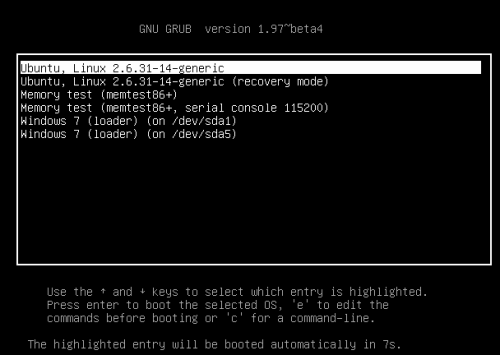
\includegraphics[totalheight=0.8\textheight]{grub.png}
}
\subsection{Installing Ubuntu}
\frame
{
	And now a live demo!
}
\section{Install Issues}
\subsection{This looks weird.}
\frame
{
	\frametitle{Oh crap, what happened? (install issues)}
	\begin{itemize}
	\item{Graphics}
	\item{Wireless}
	\end{itemize}
	Step One if you have problems: wait until you update.\\
	Step Two: Remember, Google is your best friend. If he fails you, then try the listserv.
}
\subsection{Drivers}
\frame
{
	\frametitle{Proprietary vs. Free}
	If the system doesn't automatically prompt you for drivers after installation, then you can find it at System$\Rightarrow$Administration$\Rightarrow$Hardware Drivers. \\
	Most of the free drivers should work out of the box. You may prefer free drivers, but sometimes you just have to use proprietary.
}
\section{Out of the Box Software}
\subsection{Firefox}
\frame
{
    \frametitle{Firefox}
    \begin{itemize}
    \item{Same great browser}
    \item{Firefox sync addon to keep windows and linux sessions connected}
    \end{itemize}
}
\subsection{Open Office}
\frame
{
    \frametitle{Open Office}
    \begin{itemize}
    \item{Same as windows version}
    \item{Mostly compatible with MS Office}
    \item{More compatible with .docx than some versions of MS Office}
	\item{This is what is installed on the Linux lab machines}
    \end{itemize}
}
\subsection{Empathy}
\frame
{
	\frametitle{Empathy}
	Empathy is the default Instant Messaging client in ubuntu. It is accessible through the taskbar. \\
        Many users (mostly the cool ones) prefer pidgin.
}
\frame
{
	\frametitle{Pidgin}
	\begin{itemize}
	\item{Supports AIM, MSN, yahoo, and many others}
	\item{Supports UIC's internal Instant messaging service (jabber)}
	\item{After installation, pidgin is integrated into the taskbar}
	\end{itemize}
}
\section{Installing and Uninstalling}
\subsection{aptitude}
\frame
{
	\frametitle{aptitude command}
	\begin{itemize}
	\item{aptitude search}
	\item{aptitude install}
		\begin{itemize}
		\item{a quick word about sudo access!}
		\end{itemize}
	\item{aptitude remove}
		\begin{itemize}
		\item{also needs sudo}
		\end{itemize}
	\end{itemize}
	Aptitude is good for when you know what you want to install.	
	
}
\subsection{Ubuntu Software Center}
\frame
{
	\frametitle{Ubuntu Software Center}
	Ubuntu Sofware Center is good for browsing for free software. \\
	You can also see a list of installed programs here.

}
\subsection{Locate Great Software Online}
\frame
{	
	\frametitle{DIY installations}
	\begin{itemize}
	\item{Why? when you have aptitude and U.S.C}
	\item{tar is kind of like zip}
	\item{Installing checkinstall will make your life easier}
	\item{./configure}
	\item{make}
	\item{sudo checkinstall --install}
	\end{itemize}

}
\subsection{DeLocate Great Software}
\frame
{
	\frametitle{DIY Uninstallations}
	\begin{itemize}
	\item{sudo dpkg -r packageNameGoesHere}
	\item{This command should be able to uninstall anything you installed using the 3 methods}
	\end{itemize}

}
\section{Getting Ubuntu}
\subsection{Free install cd's}
\frame
{
    \frametitle{Free install cd's}
    Use these as much as you want; share as much as you want.
}
\subsection{Download}
\frame
{
    \frametitle{Download the disk image}
    The install disk is a free download from \url{http://ubuntu.com}.\\
    Burn it.\\
    Use it.
}

\end{document}
